
\section{附录：$\rho$ 的构造与性质}
\label{sec:construction-rho}

\subsection{预备知识}
\label{subsec:rho-preliminaries}

设 $B$ 是\trForm
\[
\CC^{2n}\times\CC^{2n}\longrightarrow\RR\text{，}
\]
它由
\[
B(X_1,X_2)=\operatorname{Im}\,\omega(\overline{X}_1,X_2)
\]
来定义。

\begin{lemma}\label{thm:form-b-properties}
形式 $B$ 是 $\RR$-双线性的、对称的\trNondegenerate{}形式。此外，它满足
\[
B(iX_1,iX_2)=B(X_1,X_2)\qquad\text{并且}\qquad
B(\overline{X}_1,\overline{X}_2)=-B(X_1,X_2)\text{。}
\]
\end{lemma}

\begin{proof}
显然 $B$ 是 $\RR$-双线性的。证明它是对称的毫不费力：
\[
\begin{aligned}
B(X_2,X_1)&=\operatorname{Im}\,\omega(\overline{X}_2,X_1)\\
&=-\operatorname{Im}\,\omega(X_1,\overline{X}_2)\\
&=\operatorname{Im}\,\overline{\omega(X_1,\overline{X}_2)}\\
&=\operatorname{Im}\,\omega(\overline{X}_1,X_2)=B(X_1,X_2)\text{。}
\end{aligned}
\]
为了证明它是\trNondegenerate{}的，我们设 $X$ 对每个 $Y$ 都满足 $B(X,Y)=0$。于是我们有
\[
\operatorname{Im}\,\omega(\overline{X},Y)=0\qquad\forall Y\in\CC^{2n}\text{，}
\]
从而也有
\[
\operatorname{Im}\,\omega(\overline{X},iY)=0\qquad\forall Y\in\CC^{2n}\text{，}
\]
进而有
\[
\omega(\overline{X},Y)=0\qquad\forall Y\in\CC^{2n}\text{，}
\]
于是由 $\omega$ 是\trNondegenerate{}的可知 $\overline{X}=0$。
这两个等式也有毫不费力的证明：
\[
B(iX_1,iX_2)=\operatorname{Im}\,\omega(-i\overline{X}_1,iX_2)
=\operatorname{Im}\,\omega(\overline{X}_1,X_2)=B(X_1,X_2)
\]
是第一个，而
\[
B(\overline{X}_1,\overline{X}_2)=\operatorname{Im}\,\omega(X_1,\overline{X}_2)
=-\operatorname{Im}\,\overline{\omega(X_1,\overline{X}_2)}
=-\operatorname{Im}\,\omega(\overline{X}_1,X_2)=-B(X_1,X_2)
\]
是第二个。
\end{proof}

\begin{corollary}\label{thm:quadratic-form-q}
\trQuadraticForm{} $Q(X)=B(X,X)=\operatorname{Im}\,\omega(\overline{X},X)$ 是\trNondegenerate{}的，并且它的\trSignature{}为零。\noqed
\end{corollary}

我们所采用的术语是：\trQuadraticForm{}的\emph{\trSignature}指差
\[
\sigma(Q)=m_+(Q)-m_-(Q)\text{，}
\]
其中 $m_+$、相应地 $m_-$，是使 $Q$ 在其上\trPositiveDefinite{}、相应地\trNegativeDefinite{}的子空间的最大维数（$m_-$ 就是在\trCriticalPoint{}的语境中所说的那个\trIndex）。

\begin{lemma}\label{thm:b-orthogonal-eigenspaces}
设 $\lambda$ 与 $\mu$ 是 $A$ 的两个\trEigenvalue。若 $\overline{\lambda}\,\mu\neq1$，那么\trGeneralizedEigenspace{} $E_\lambda$ 与 $E_\mu$ 关于 $B$ 是\trOrthogonal{}的。
\end{lemma}

\begin{proof}
这是\cref{thm:sp-orthogonal-eigenspaces}的一个直接推论：若 $X_1\in E_\lambda$ 且 $X_2\in E_\mu$，则 $\overline{X}_1\in E_{\overline{\lambda}}$，从而 $\omega(\overline{X}_1,X_2)=0$。
\end{proof}

\begin{corollary}\label{thm:restriction-signature-zero}
\begin{enumerate}[label=(\arabic*)]
\item 设 $\lambda\in S^1$；那么 $B$ 与 $Q$ 在 $E_\lambda$ 上的限制都是\trNondegenerate{}的。
\item 设 $\lambda\in\CC-S^1$；那么 $B$ 与 $Q$ 在 $E_\lambda\oplus E_{1/\overline{\lambda}}$ 上的限制都是\trNondegenerate{}的。此外，$Q$ 在这个子空间上的限制的\trSignature{}为零。
\end{enumerate}
\end{corollary}

\begin{proof}
唯一值得验证的断言是关于\trSignature{}的那一条。我们知道，$\omega$ 在 $E_\lambda\oplus E_{1/\lambda}$ 上的限制是\trNondegenerate{}的（\cref{thm:sp-eigenspace-corollary}），并且这两个\trGeneralizedEigenspace{}都是\trIsotropic{}的。因此我们可以找到 $E_\lambda$ 的一组基 $(X_1,\dotsc,X_k)$ 与 $E_{1/\overline{\lambda}}$ 的一组基 $(Y_1,\dotsc,Y_k)$，使得 $(X_1,\dotsc,X_k,\overline{Y}_1,\dotsc,\overline{Y}_k)$ 是 $E_\lambda\oplus E_{1/\lambda}$ 的一组\trSymplectic{}基。\footnote{译注：原书此处印作“$E_{\overline{\lambda}}$ 的一组基”；按下文关于 $u_j$、$v_j$ 的计算（要求 $\omega(\overline{Y}_j,X_k)$ 给出 $\delta_{j,k}$），这组基应取自 $E_{1/\overline{\lambda}}$（从而 $\overline{Y}_j\in E_{1/\lambda}$），系原书笔误，径改。——译者注}令
\[
u_j=X_j+iY_j,\qquad v_j=X_j-iY_j\text{。}
\]
于是我们有
\[
\begin{aligned}
B(u_j,u_k)&=B(X_j+iY_j,X_k+iY_k)\\
&=B(iY_j,X_k)+B(iY_k,X_j)\\
&=\operatorname{Im}\,\omega(-i\overline{Y}_j,X_k)+\operatorname{Im}\,\omega(-i\overline{Y}_k,X_j)\\
&=2\delta_{j,k}\text{，}
\end{aligned}
\]
从而 $Q$ 在由诸 $u_j$ 生成的子空间上是\trPositiveDefinite{}的，并且
\[
\begin{aligned}
B(u_j,v_k)&=B(X_j+iY_j,X_k-iY_k)\\
&=B(iY_j,X_k)-B(iY_k,X_j)\\
&=0\text{，}
\end{aligned}
\]
从而由诸 $u_j$ 生成的子空间与由诸 $v_j$ 生成的子空间是\trOrthogonal{}的。最后，
\[
\begin{aligned}
B(v_j,v_k)&=B(X_j-iY_j,X_k-iY_k)\\
&=-B(iY_j,X_k)-B(iY_k,X_j)\\
&=-2\delta_{j,k}\text{，}
\end{aligned}
\]
从而 $Q$ 在由诸 $v_j$ 生成的子空间上是负的，因而\trSignature{}为零。
\end{proof}

\subsection{$\rho$ 的定义}
\label{subsec:rho-definition}

现在让我们来定义映射 $\rho$。若 $\lambda\in S^1-\RR$ 是一个\trEigenvalue，那么我们可以把\trGeneralizedEigenspace
\[
E_\lambda=E_\lambda^+\oplus E_\lambda^-
\]
写成 $\CC^{2n}$ 的两个实向量子空间之和，形式 $Q$ 在这两个子空间上分别\trPositiveDefinite{}与\trNegativeDefinite{}。由于 $Q(iX)=Q(X)$，这两个子空间在乘以 $i$ 下稳定，而且事实上是 $\CC^{2n}$ 的\emph{复}向量子空间。\footnote{译注：原书由 $Q(iX)=Q(X)$（$Q$ 在乘 $i$ 下不变）径断“这两个子空间在乘 $i$ 下稳定”；然 $Q$ 之不变只保证子空间经 $i$ 替换后正、负号不变，并不保证任意取定的正（或负）子空间本身复稳定。反例：$Q(z,w)=|z|^{2}-|w|^{2}$，取 $P=\{(z,\varepsilon\overline{z})\}$（$\varepsilon<1$ 时 $Q$ 在 $P$ 上\trPositiveDefinite），则 $i\cdot(z,\varepsilon\overline{z})=(iz,i\varepsilon\overline{z})\notin P$。故 $E_\lambda^{\pm}$ 应取自相应的 Hermitian 型的正、负谱空间（如此方自动复稳定），再得分解 $E_\lambda=E_\lambda^{+}\oplus E_\lambda^{-}$。此处照原书排印，存疑备案。——译者注}

我们令 $m_+(\lambda)$ 与 $m_-(\lambda)$ 为这些空间的复维数，
\[
m_+(\lambda)=\dim_\CC E_\lambda^+,\qquad m_-(\lambda)=\dim_\CC E_\lambda^-\text{，}
\]
于是
\[
m_+(\lambda)+m_-(\lambda)=\dim_\CC E_\lambda=m(\lambda)\text{，}
\]
即 $\lambda$ 的\trMultiplicity。这样，我们就把\trEigenvalue{} $\lambda$ 的\emph{\trSignature}定义为
\[
\sigma(\lambda)=m_+(\lambda)-m_-(\lambda)\text{。}
\]

回想一下，$-1$ 作为（可能的）\trEigenvalue{}的\trMultiplicity{}是偶数，因为 $E_{-1}$ 是\trSymplectic{}的（\cref{thm:sp-eigenspace-corollary}），从而诸负实\trEigenvalue{}的\trMultiplicity{}之和是偶数，也就是说，
\[
m_0=\sum_{\lambda\in\operatorname{Spec}(A)\cap\RR_-}m(\lambda)\in 2\NN\text{。}
\]
因此，我们最终可以设置
\[
\rho(A)=(-1)^{m_0/2}\prod_{\lambda\in\operatorname{Spec}(A)\cap(S^1-\RR)}\lambda^{m_+(\lambda)}\text{。}
\]
这就是\cref{thm:rho-map-properties}所宣布的那个映射，正如我们将要证明的。我们首先注意到，其实只用带正虚部的诸\trEigenvalue{}也可以。

\begin{proposition}\label{thm:rho-positive-imag}
\[
\rho(A)=(-1)^{m_0/2}\prod_{\substack{\lambda\in\operatorname{Spec}(A)\cap S^1\\ \operatorname{Im}(\lambda)>0}}\lambda^{\sigma(\lambda)}\text{。}
\]
\end{proposition}

\begin{proof}
我们已经说过（\cref{thm:sp-conjugate-isomorphism}），$X\mapsto\overline{X}$ 是从 $E_\lambda$ 到 $E_{\overline{\lambda}}$ 上的一个实\trVectorSpace{}\trIsomorphism。由于 $Q(\overline{X})=-Q(X)$，故对 $\lambda\in S^1$ 有
\[
\left\{\begin{array}{l}
m_+(\overline{\lambda})=m_-(\lambda)\\
m_-(\overline{\lambda})=m_+(\lambda)\\
\sigma(\overline{\lambda})=-\sigma(\lambda)\text{，}
\end{array}\right.
\]
从而
\[
\lambda^{m_+(\lambda)}\cdot\overline{\lambda}^{\,m_+(\overline{\lambda})}
=\lambda^{\sigma(\lambda)}=\overline{\lambda}^{\,\sigma(\overline{\lambda})}\text{。}
\]
在 $\rho$ 的定义中把绝对值为 $1$ 的诸\trEigenvalue{}归成对 $(\lambda,\overline{\lambda})$，就得到所陈述的公式。\footnote{译注：末项本译初版误衍一枚负号（印作 $\overline{\lambda}^{\,-\sigma(\overline{\lambda})}$）；经页图实证（p-213，印刷 205），原书径作 $\overline{\lambda}^{\,\sigma(\overline{\lambda})}$，兹删负号、照原书复原。等式本身成立：由上方 $\sigma(\overline{\lambda})=-\sigma(\lambda)$ 与 $|\lambda|=1$（$\overline{\lambda}=1/\lambda$）得 $\overline{\lambda}^{\,\sigma(\overline{\lambda})}=\overline{\lambda}^{-\sigma(\lambda)}=(1/\lambda)^{-\sigma(\lambda)}=\lambda^{\sigma(\lambda)}$。——译者注}
\end{proof}

\subsection{$\rho$ 的性质}
\label{subsec:rho-properties}

现在让我们开始验证 $\rho$ 的各个所期望的性质，也就是说，证明\cref{thm:rho-map-properties}。

\textbf{$\rho$ 的连续性}

设 $(A_k)_{k\in\NN}$ 是 $\mathrm{Sp}(2n;\RR)$ 中一列\trConvergence{}于矩阵 $A\in\mathrm{Sp}(2n)$ 的矩阵。我们将要证明，由诸 $\rho(A_k)$ 组成的序列\trConvergence{}于 $\rho(A)$。显然，只需对 $(A_k)$ 的一个子序列证明这一点。我们将要用到\trEigenvalue{}连续依赖于矩阵的系数这一事实，这个经典事实可以陈述如下。\nolinebreak\footnote{这个证明留给有意愿的读者当作练习；在\cref{ex:ch14-043-rouche-eigenvalue-continuity}中，我们给出了一个基于\trRouche{}定理的证明。}

\begin{proposition}\label{thm:eigenvalue-continuity}
设 $(A_k)_{k\in\NN}$ 是一列趋于极限 $A$ 的 $m\times m$ 方阵。设 $\lambda_1,\dotsc,\lambda_m$ 是 $A$ 的诸\trEigenvalue，按其\trMultiplicity{}重复。那么，存在 $A_k$ 的诸\trEigenvalue{}的一个编号 $\lambda^k_1,\dotsc,\lambda^k_m$，使得
\[
\forall i\in[1,m]\qquad\lim_{k\to+\infty}\lambda^k_i=\lambda_i\text{。}
\]
\end{proposition}

我们还需要一个关于\trGeneralizedEigenspace{}的连续性的结果。

\begin{proposition}\label{thm:eigenspace-continuity}
在同样的假设下，设 $\lambda$ 是 $A$ 的一个\trEigenvalue。那么，必要时抽取一个子序列之后，
\[
\lim_{k\to+\infty}\bigoplus_{\substack{\lim\lambda^k_i=\lambda\\ i\neq j\Rightarrow\lambda^k_i\neq\lambda^k_j}}E_{\lambda^k_i}(A_k)=E_\lambda(A)\text{。}
\]
\end{proposition}

在这个陈述中，一列具有同一维数的（$\CC^m$ 的）向量子空间向一个具有这一维数的子空间的\trConvergence，其定义（也就是说，作为相应\trGrassmann\trManifold{}中的\trConvergence）为：$\lim V_k=V$，如果对每个 $k$ 都存在 $V_k$ 的一组\trUnitary{}基 $\mathfrak{B}_k$，使得序列 $\mathfrak{B}_k$ \trConvergence{}于 $V$ 的一组基 $\mathfrak{B}$。

\begin{proof}[\cref{thm:eigenspace-continuity}的证明]
设 $\lambda^k_1,\lambda^k_2,\dotsc,\lambda^k_{r_k}$ 表示其\trGeneralizedEigenspace{}出现在这个\trDirectSum{}中的 $A_k$ 的那些（相异的）\trEigenvalue。由\cref{thm:eigenvalue-continuity}，我们知道它们的\trMultiplicity{}之和就是极限 $\lambda$ 的\trMultiplicity。设 $V_k$ 是这个\trDirectSum，并注意到
\[
V_k\subset\operatorname{Ker}(A_k-\lambda^k_1\mathrm{Id})^{m(\lambda^k_1)}
(A_k-\lambda^k_2\mathrm{Id})^{m(\lambda^k_2)}\cdots
(A_k-\lambda^k_{r_k}\mathrm{Id})^{m(\lambda^k_{r_k})}\text{。}
\]
事实上，$(A_k-\lambda^k_j\mathrm{Id})^{m(\lambda^k_j)}$ 在\trGeneralizedEigenspace{} $E_{\lambda^k_j}(A_k)$ 上为零（由\trGeneralizedEigenspace{}的定义）。因此，若 $v_k\in V_k$ 是一列\trConvergence{}于 $v$ 的向量，则
\[
(A-\lambda\mathrm{Id})^{m(\lambda)}v=0\text{，}
\]
从而 $v\in E_\lambda(A)$。
\end{proof}

从\cref{thm:eigenvalue-continuity}出发，我们不难推出下面这个有用的结果。

\begin{proposition}\label{thm:signature-continuity}
若 $(V_k)_{k\in\NN}$ 是一列\trConvergence{}于子空间 $V$ 的、$\CC^m$ 的具有同一维数的向量子空间，且 $Q$ 是 $\CC^m$ 上的一个\trQuadraticForm，它在每个 $V_k$ 上以及在 $V$ 上的限制都是\trNondegenerate{}的，那么对充分大的 $k$，$Q|_{V_k}$ 的\trSignature{}是常数，并且等于 $Q|_V$ 的\trSignature。
\end{proposition}

\begin{proof}
我们选取 $V_k$ 的一列\trConvergence{}于 $V$ 的一组\trUnitary{}基的\trUnitary{}基。$Q$ 在 $V_k$ 上的限制的矩阵趋于 $Q$ 在 $V$ 上的限制的矩阵。因此，把正\trEigenvalue{}按\trMultiplicity{}计数，其个数对充分大的 $k$ 而言是常数。
\end{proof}

现在让我们来证明 $\rho$ 的连续性。设 $(A_k)_{k\in\NN}$ 是一列\trConvergence{}于 $A\in\mathrm{Sp}(2n)$ 的\trSymplectic{}矩阵，并设 $\lambda\in S^1\cap\{\operatorname{Im}(z)>0\}$ 是 $A$ 的一个\trEigenvalue。沿用上面所用的记号，我们令
\[
E_\lambda(A)=\lim_{k\to+\infty}E_{\lambda^k_1}(A_k)\oplus\dotsb\oplus E_{\lambda^k_{r_k}}(A_k)\text{。}
\]
\trEigenvalue{} $\lambda$ 既可以用一列由 $A_k$ 的位于\trCircle{}上的\trEigenvalue{}组成的序列 $(\lambda^k)_{k\in\NN}$ 来逼近，也可以用一列由\trCircle{}之外的数组成的序列 $(\mu^k)_{k\in\NN}$ 来逼近，而在后一种情形，它还可以用序列 $(1/\overline{\mu}^k)_{k\in\NN}$ 来逼近。\cref{fig:rho-circle-approx}所示即此。

\begin{figure}[htbp]
\centering
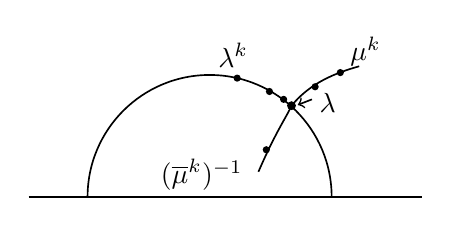
\begin{tikzpicture}[line width=0.6pt]
  \draw (-2.3,0) -- (2.7,0);
  \draw (1.55,0) arc (0:180:1.55);
  \fill (0.35,1.51) circle (1.3pt);
  \node at (0.3,1.8) {$\lambda^k$};
  \fill (0.76,1.34) circle (1.3pt);
  \fill (0.94,1.24) circle (1.3pt);
  \fill (1.04,1.16) circle (1.6pt);
  \node at (1.5,1.2) {$\lambda$};
  \draw[->] (1.3,1.24) -- (1.12,1.17);
  \draw (0.62,0.32) .. controls (0.85,0.85) and (0.98,1.02) .. (1.04,1.16)
        .. controls (1.24,1.4) and (1.5,1.55) .. (1.9,1.66);
  \fill (0.72,0.6) circle (1.3pt);
  \fill (1.34,1.4) circle (1.3pt);
  \fill (1.66,1.58) circle (1.3pt);
  \node at (1.98,1.85) {$\mu^k$};
  \node at (-0.1,0.28) {$(\overline{\mu}^k)^{-1}$};
\end{tikzpicture}
\caption{}
\label{fig:rho-circle-approx}
\end{figure}

设 $\lambda^k_1,\dotsc,\lambda^k_{s_k}$（其中 $s_k\le r_k$）是对充分大的 $k$ 而言位于\trCircle{}上的那些\trEigenvalue。下面是\cref{thm:signature-continuity}的一个推论。

\begin{corollary}\label{thm:rho-circle-limit}
\[
\lim_{k\to+\infty}(\lambda^k_1)^{\sigma(\lambda^k_1)}\cdots
(\lambda^k_{s_k})^{\sigma(\lambda^k_{s_k})}=\lambda^{\sigma(\lambda)}\text{。}
\]
\end{corollary}

\begin{proof}
当 $s_k=r_k$ 时，这是\cref{thm:signature-continuity}的一个直接推论，因为此时对充分大的 $k$ 有
\[
\sigma(\lambda^k_1)+\dotsb+\sigma(\lambda^k_{s_k})=\sigma(\lambda)\text{，}
\]
这就给出了所要的结果。若 $s_k<r_k$，那么诸\trEigenvalue{} $\lambda^k_{s_k+1},\dotsc,\lambda^k_{r_k}$ 可以归成具有同一\trMultiplicity{}的对 $\mu,\overline{\mu}^{-1}$（如\cref{fig:rho-circle-approx}所示）。然而，由\cref{thm:restriction-signature-zero}，$Q$ 在 $E_\mu(A_k)\oplus E_{\overline{\mu}^{-1}}(A_k)$ 上的\trSignature{}为零。诸\trSignature{}之间的关系再次得到满足，推论得证。
\end{proof}

为了结束连续性的证明，我们需要分析 $A_k$ 的那些趋于 $A$ 的一个实\trEigenvalue{} $\lambda$ 的\trEigenvalue{}序列。我们从 $\lambda>0$ 的情形开始。若 $\lambda\neq1$，那么诸 $\lambda^k_i$ 与 $\lambda$ 在 $\rho$ 的定义中不起任何作用。若 $\lambda=1$，那么在 $\rho$ 的定义中起作用的序列，只是那些对充分大的 $k$ 落在 $S^1\cap\{\operatorname{Im}(z)>0\}$ 中的序列（\cref{fig:rho-near-one}）。对其中的每一个，都有
\[
\lim_{k\to+\infty}(\lambda^k)^{\sigma(\lambda^k)}=1
\qquad\text{因为}\qquad\lim_{k\to+\infty}\lambda^k=1\text{。}
\]

\begin{figure}[htbp]
\centering
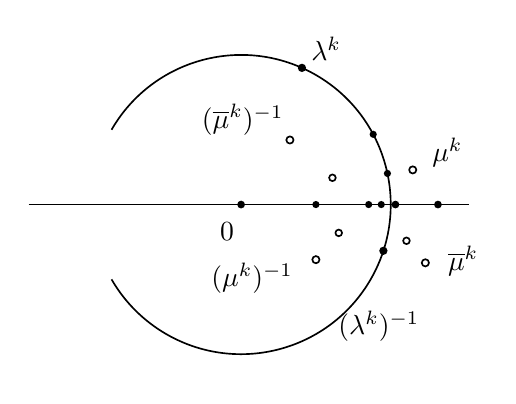
\begin{tikzpicture}[line width=0.6pt]
  \draw (150:1.9) arc (150:-150:1.9);
  \draw (-2.7,0) -- (2.9,0);
  \fill (0,0) circle (1.4pt);
  \node at (-0.18,-0.34) {$0$};
  \fill (0.95,0) circle (1.3pt);
  \fill (1.62,0) circle (1.3pt);
  \fill (1.78,0) circle (1.3pt);
  \fill (1.96,0) circle (1.4pt);
  \fill (2.5,0) circle (1.4pt);
  \fill (66:1.9) circle (1.5pt);
  \node at (1.08,1.98) {$\lambda^k$};
  \fill (28:1.9) circle (1.3pt);
  \fill (12:1.9) circle (1.3pt);
  \fill (-18:1.9) circle (1.5pt);
  \node at (1.75,-1.55) {$(\lambda^k)^{-1}$};
  \draw (0.62,0.82) circle (1.3pt);
  \node at (0.02,1.08) {$(\overline{\mu}^k)^{-1}$};
  \draw (1.16,0.34) circle (1.2pt);
  \draw (1.24,-0.36) circle (1.2pt);
  \draw (2.18,0.44) circle (1.3pt);
  \node at (2.62,0.66) {$\mu^k$};
  \draw (2.1,-0.46) circle (1.2pt);
  \draw (2.34,-0.74) circle (1.3pt);
  \node at (2.82,-0.72) {$\overline{\mu}^k$};
  \draw (0.95,-0.7) circle (1.3pt);
  \node at (0.14,-0.94) {$(\mu^k)^{-1}$};
\end{tikzpicture}
\caption{}
\label{fig:rho-near-one}
\end{figure}

现在让我们转向 $\lambda<0$ 的情形（\cref{fig:rho-negative-real}与\cref{fig:rho-minus-one}）。设：
\begin{itemize}
\item （如上）$\lambda^k_1,\dotsc,\lambda^k_{s_k}$ 是 $A_k$ 的那些对充分大的 $k$ 属于 $S^1\cap\{\operatorname{Im}(z)>0\}$ 的\trEigenvalue{}序列（如果至少存在一个，那么 $\lambda=-1$）；
\item $\lambda^k_{s_k+1},\dotsc,\lambda^k_{t_k}$ 是实的序列；
\item $\lambda^k_{t_k+1},\dotsc,\lambda^k_{r_k}$ 是其余的序列。
\end{itemize}
我们将证明下面的结果。

\begin{proposition}\label{thm:rho-negative-real}
\[
\lim_{k\to+\infty}(\lambda^k_1)^{\sigma(\lambda^k_1)}\cdots
(\lambda^k_{s_k})^{\sigma(\lambda^k_{s_k})}\cdot
(-1)^{(m(\lambda^k_{s_k+1})+\dotsb+m(\lambda^k_{t_k}))/2}=(-1)^{m(\lambda)/2}\text{。}
\]
\end{proposition}

\begin{proof}
若 $\lambda\neq-1$，那么 $s_k=0$，而诸\trEigenvalue{} $\lambda^k_{t_k+1},\dotsc,\lambda^k_{r_k}$ 可以归成四元组 $\mu,1/\mu,\overline{\mu},1/\overline{\mu}$（\cref{fig:rho-negative-real}），于是
\[
m(\mu)+m(1/\mu)+m(\overline{\mu})+m(1/\overline{\mu})=4m(\mu)\text{。}
\]
因此，对充分大的 $k$，\trEigenvalue{}的连续性（\cref{thm:eigenvalue-continuity}）蕴含
\[
\frac{m(\lambda)}{2}=\sum_{i=1}^{r_k}\frac{m(\lambda^k_i)}{2}
\qquad\text{与}\qquad
\sum_{i=1}^{t_k}\frac{m(\lambda^k_i)}{2}
\]
有相同的奇偶性，\footnote{译注：此处（以及\cref{thm:rho-negative-real}的陈述）把 $m(\lambda)/2$ 当作可谈奇偶性的整数；然对负实\trEigenvalue{} $\lambda\neq-1$，$1/\lambda$ 亦是\trEigenvalue{}且与 $\lambda$ 同\trMultiplicity，单簇的 $m(\lambda)$ 可为奇数，此时 $m(\lambda)/2$ 非整数、奇偶性无定义。反例：取 $B_\varepsilon=-2R_\varepsilon$（$R_\varepsilon$ 为转角 $\varepsilon$ 的旋转）与 $A_\varepsilon=\operatorname{diag}(B_\varepsilon,B_\varepsilon^{-T})\in\mathrm{Sp}(4)$，则 $\varepsilon\to0$ 时 $A_\varepsilon$ 无任何实\trEigenvalue，命题左端为 $(-1)^{0}=1$，而右端为 $(-1)^{m(-2)/2}=-1$。应把 $\lambda$ 与 $1/\lambda$ 两簇的总\trMultiplicity{}合并之后再谈偶性（合并后 $(m(\lambda)+m(1/\lambda))/2=m(\lambda)$ 恒为整数）。$\lambda=-1$ 为自反簇（单簇即全簇，且 $m(-1)$ 为偶数），原论证在该情形有效。此处照原书排印，存疑备案。——译者注}这就结束了这种情形的证明。

\begin{figure}[htbp]
\begin{minipage}[b]{0.46\textwidth}
\centering
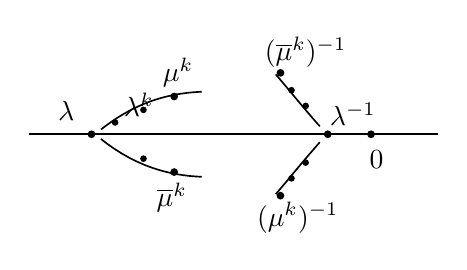
\begin{tikzpicture}[line width=0.6pt]
  \draw (-0.8,0) -- (4.4,0);
  \fill (0,0) circle (1.4pt);
  \node at (-0.32,0.3) {$\lambda$};
  \draw (0.12,0.06) .. controls (0.5,0.36) and (0.9,0.52) .. (1.4,0.54);
  \draw (0.12,-0.06) .. controls (0.5,-0.36) and (0.9,-0.52) .. (1.4,-0.54);
  \fill (0.3,0.15) circle (1.2pt);
  \node at (0.6,0.38) {$\lambda^k$};
  \fill (0.66,0.31) circle (1.2pt);
  \fill (1.05,0.48) circle (1.4pt);
  \node at (1.1,0.78) {$\mu^k$};
  \fill (0.66,-0.31) circle (1.2pt);
  \fill (1.05,-0.48) circle (1.4pt);
  \node at (1.02,-0.8) {$\overline{\mu}^k$};
  \fill (3.0,0) circle (1.4pt);
  \node at (3.32,0.26) {$\lambda^{-1}$};
  \draw (2.9,0.1) .. controls (2.62,0.42) and (2.48,0.6) .. (2.34,0.76);
  \draw (2.9,-0.1) .. controls (2.62,-0.42) and (2.48,-0.6) .. (2.34,-0.76);
  \fill (2.72,0.36) circle (1.2pt);
  \fill (2.54,0.56) circle (1.2pt);
  \fill (2.4,0.78) circle (1.4pt);
  \node at (2.72,1.04) {$(\overline{\mu}^k)^{-1}$};
  \fill (2.72,-0.36) circle (1.2pt);
  \fill (2.54,-0.56) circle (1.2pt);
  \fill (2.4,-0.78) circle (1.4pt);
  \node at (2.62,-1.06) {$(\mu^k)^{-1}$};
  \fill (3.55,0) circle (1.4pt);
  \node at (3.62,-0.32) {$0$};
\end{tikzpicture}
\caption{}
\label{fig:rho-negative-real}
\end{minipage}\hfill
\begin{minipage}[b]{0.50\textwidth}
\centering
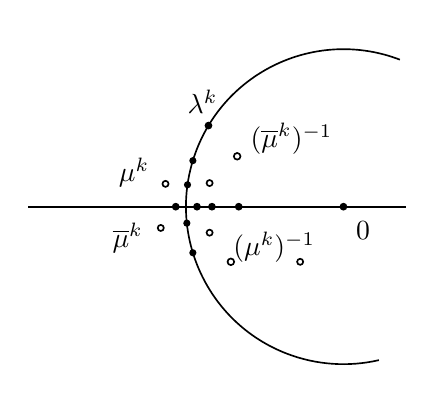
\begin{tikzpicture}[line width=0.6pt]
  \draw (-4.0,0) -- (0.8,0);
  \draw (69:2.0) arc (69:283:2.0);
  \fill (0,0) circle (1.4pt);
  \node at (0.25,-0.3) {$0$};
  \fill (149:2.0) circle (1.4pt);
  \node at (-1.79,1.33) {$\lambda^k$};
  \fill (163:2.0) circle (1.3pt);
  \fill (172:2.0) circle (1.3pt);
  \fill (186:2.0) circle (1.3pt);
  \fill (197:2.0) circle (1.3pt);
  \fill (-2.13,0) circle (1.4pt);
  \fill (-1.86,0) circle (1.4pt);
  \fill (-1.67,0) circle (1.4pt);
  \fill (-1.33,0) circle (1.4pt);
  \draw (-2.26,0.29) circle (1.1pt);
  \node at (-2.66,0.44) {$\mu^k$};
  \draw (-2.32,-0.27) circle (1.1pt);
  \node at (-2.74,-0.4) {$\overline{\mu}^k$};
  \draw (-1.70,0.30) circle (1.1pt);
  \draw (-1.35,0.64) circle (1.2pt);
  \node at (-0.66,0.86) {$(\overline{\mu}^k)^{-1}$};
  \draw (-1.70,-0.33) circle (1.1pt);
  \draw (-1.43,-0.70) circle (1.2pt);
  \node at (-0.88,-0.52) {$(\mu^k)^{-1}$};
  \draw (-0.55,-0.70) circle (1.1pt);
\end{tikzpicture}
\caption{}
\label{fig:rho-minus-one}
\end{minipage}
\end{figure}

若 $\lambda=-1$，那么诸\trEigenvalue{} $\lambda^k_{t_k+1},\dotsc,\lambda^k_{r_k}$ 或者是诸共轭 $\overline{\lambda}^k_1,\dotsc,\overline{\lambda}^k_{s_k}$，或者是四元组 $\mu,1/\mu,\overline{\mu},1/\overline{\mu}$（\cref{fig:rho-minus-one}）。\footnote{译注：原书此处印作“$\lambda_{t_k+1},\dotsc,\lambda_{r_k}$”，脱上标 $k$；疑应为“$\lambda^k_{t_k+1},\dotsc,\lambda^k_{r_k}$”（同句并列的 $\overline{\lambda}^k_1,\dotsc,\overline{\lambda}^k_{s_k}$ 以及下文诸式均带上标 $k$，所指即 $A_k$ 的诸\trEigenvalue{}序列），系原书排版脱字，此处径补。——译者注}这一次，对充分大的 $k$，并且模 $2$ 而言，我们有
\[
\begin{aligned}
\frac{m(\lambda)}{2}
&\equiv\sum_{i=1}^{s_k}\frac{m(\lambda^k_i)}{2}
+\sum_{i=1}^{s_k}\frac{m(\overline{\lambda_i^k})}{2}
+\sum_{i=s_k+1}^{t_k}\frac{m(\lambda^k_i)}{2}\\
&\equiv\sum_{i=1}^{s_k}m(\lambda^k_i)+\sum_{i=s_k+1}^{t_k}\frac{m(\lambda^k_i)}{2}\\
&\equiv\sum_{i=1}^{s_k}\sigma(\lambda^k_i)+\sum_{i=s_k+1}^{t_k}\frac{m(\lambda^k_i)}{2}\text{，}
\end{aligned}
\]
因为 $m$ 与 $\sigma$ 有相同的奇偶性。这就是所要陈述的结果。
\end{proof}

这个结果（也就是\cref{thm:rho-circle-limit}与\cref{thm:rho-negative-real}）结束了 $\rho$ 的连续性的证明。\noqed

现在让我们来证明，所得到的这个连续映射 $\rho$ 满足\cref{thm:rho-map-properties}中宣布的全部性质。

\par\nopagebreak
\textbf{自然性}\nopagebreak

矩阵 $TAT^{-1}$ 与 $A$ 有相同的\trSpectrum，包括诸\trMultiplicity。此外，诸\trGeneralizedEigenspace{}经由
\[
E^{TAT^{-1}}_\lambda=T(E^A_\lambda)
\]
相互对应。最后，由于 $T$ 并不是一个随随便便的\trInvertible{}矩阵，而是 $\mathrm{Sp}(2n;\RR)$ 的一个元素，它保持\trSymplecticForm{} $\omega$ 以及一切由它导出的东西。特别地，$Q(T(X))=Q(X)$，于是
\[
m^{TAT^{-1}}_\pm(\lambda)=m^A_\pm(\lambda)
\qquad\text{并且最终有 }\rho(TAT^{-1})=\rho(A)\text{。}
\]
\noqed

\par\nopagebreak
\textbf{乘积}\nopagebreak

$\left(\begin{smallmatrix}A&0\\0&B\end{smallmatrix}\right)$ 的\trSpectrum{}是 $A$ 与 $B$ 的\trSpectrum{}的并（连同\trMultiplicity），并且类似地（约定：若 $\lambda$ 不是\trEigenvalue，则 $E_\lambda=0$），
\[
E_\lambda\begin{pmatrix}A&0\\0&B\end{pmatrix}=E_\lambda(A)\oplus E_\lambda(B)\text{。}
\]
诸 $m_\pm$ 也相加，因此
\[
\rho\begin{pmatrix}A&0\\0&B\end{pmatrix}=\rho(A)\rho(B)\text{。}
\]
\noqed

\par\nopagebreak
\textbf{正规化}\nopagebreak

这条性质（当诸\trEigenvalue{}全为实时 $\rho=\pm1$）是 $\rho$ 的定义的一个直接推论。\noqed

\par\nopagebreak
\textbf{行列式}\nopagebreak

设 $A\in\mathrm{Sp}(2n;\RR)\cap\mathrm{O}(2n)=\mathrm{U}(n)$，则
\[
A=\begin{pmatrix}M&-N\\N&M\end{pmatrix}\text{，}
\]
它被等同于 $U=M+iN\in\mathrm{U}(n)$。首先注意，$A$ 的诸\trEigenvalue{}的确就是 $U$ 的诸\trEigenvalue。一方面，我们有
\[
U(z)=\lambda z\Longrightarrow A\binom{z}{-iz}=\lambda\binom{z}{-iz}
\]
而另一方面，我们有
\[
\begin{pmatrix}M&-N\\N&M\end{pmatrix}\binom{v}{w}=\lambda\binom{v}{w}
\Longrightarrow(M+iN)(v+iw)=\lambda(v+iw)
\]
（倘若碰巧 $v+iw=0$，那么有 $(M-iN)v=\lambda v$，从而 $\overline{\lambda}$ 确是 $U$ 的一个\trEigenvalue。\footnote{译注：原书此处印作“$(M+iN)v=\lambda v$，从而 $\lambda$ 确是 $U$ 的一个\trEigenvalue”。按所设 $v+iw=0$（即 $w=iv$）代入，实得 $(M-iN)v=\lambda v$；再取共轭即知 $\overline{\lambda}$（而非 $\lambda$）是 $U=M+iN$ 的\trEigenvalue，系原书笔误，径改。——译者注}）特别地，正如 $U$ 的诸\trEigenvalue{}那样（因为它们是同一批），$A$ 的诸\trEigenvalue{}都是 $S^1$ 的元素。

\begin{lemma}\label{thm:unitary-multiplicities}
设 $A\in\mathrm{Sp}(2n;\RR)\cap\mathrm{O}(2n)=\mathrm{U}(n)$，并设 $\lambda$ 是 $A$ 的一个非实\trEigenvalue。那么
\[
m^A_+(\lambda)=m^U(\lambda)\qquad\text{并且}\qquad m^A(-1)=2m^U(-1)\text{。}
\]
\end{lemma}

\begin{proof}
矩阵 $A$ 与 $U$ 在 $\CC$ 上\trDiagonalizable，因此诸\trGeneralizedEigenspace{} $E_\lambda$ 不过是通常的\trEigenspace。设 $J_0$ 是\trComplexStructure
\[
J_0=\begin{pmatrix}0&-\mathrm{Id}\\\mathrm{Id}&0\end{pmatrix}\text{，}
\]
于是 $J_0^2=-\mathrm{Id}$，$AJ_0=J_0A$，并且 $\omega(X,J_0Y)=(X,Y)$——即 $\RR^{2n}$ 上的\trInnerProduct。由于 $A$ 与 $J_0$ 交换，我们有
\[
J_0(E^A_\lambda)=E^A_\lambda\text{。}
\]
此外，$J_0\in\mathrm{Sp}(2n;\RR)\cap\mathrm{O}(2n)$ 在 $\CC$ 上也\trDiagonalizable，它的\trEigenvalue{}是 $i$ 与 $-i$，各具有\trMultiplicity{} $n$，而它的\trEigenspace{}是
\[
E^{J_0}_i=\Bigl\{\binom{x}{ix}\;\Bigm|\;x\in\CC^n\Bigr\}
\qquad\text{与}\qquad
E^{J_0}_{-i}=\Bigl\{\binom{x}{-ix}\;\Bigm|\;x\in\CC^n\Bigr\}\text{。}
\]
特别地，对 $v\in E^{J_0}_i$，我们有
\[
\omega(\overline{v},v)=\omega(\overline{v},-iJ_0v)
=-i\,\omega(\overline{v},J_0v)
=-i\bigl(\|\operatorname{Re}v\|^2+\|\operatorname{Im}v\|^2\bigr)\text{，}
\]
从而 $Q$ 在 $E^{J_0}_i$ 上是\trNegativeDefinite{}的。一个类似的计算表明，它在 $E^{J_0}_{-i}$ 上是\trPositiveDefinite{}的。由此可见，$A$ 的诸\trEigenspace{}满足
\[
E^+_\lambda=E_\lambda\cap E^{J_0}_{-i}\text{，}\qquad
E^-_\lambda=E_\lambda\cap E^{J_0}_{i}\text{。}
\]
因此，
\[
\begin{aligned}
E^+_\lambda
&=\Bigl\{\binom{x}{-ix}\in\CC^{2n}\;\Bigm|\;
\begin{pmatrix}M&-N\\N&M\end{pmatrix}\binom{x}{-ix}=\lambda\binom{x}{-ix}\Bigr\}\\
&=\bigl\{x\in\CC^n\mid(M+iN)x=\lambda x\bigr\}\text{，}
\end{aligned}
\]
这恰好就是矩阵 $U$ 关于 $\lambda$ 的\trEigenspace。因此，我们确实有 $m^A_+(\lambda)=m^U(\lambda)$。\trEigenvalue{} $-1$ 的情形可以以类似的方式处理：我们可以验证
\[
\binom{v}{w}\in E^A_{-1}\cap\RR^{2n}\Longleftrightarrow(v+iw)\in E^U_{-1}\text{，}
\]
于是 $A$ 与 $U$ 关于\trEigenvalue{} $-1$ 的诸\trEigenspace{}作为实\trVectorSpace{}是\trIsomorphic{}的，并且
\[
m^A(-1)=\dim_\RR\bigl(E^A_{-1}\cap\RR^{2n}\bigr)=\dim_\RR E^U_{-1}
=2\dim_\CC E^U_{-1}=2m^U(-1)
\]
……这就完成了引理的证明……
\end{proof}

从而也就证明了 $\rho(A)=\det\nolimits_\CC(U)$。\footnote{译注：按本节约定推演，本段的行列式性质与\cref{thm:rho-map-properties}的性质 (3) 相抵触：取 $n=1$、$A=R_\theta$（此时 $U=M+iN=e^{i\theta}$），则 $\lambda=e^{i\theta}$ 的特征向量 $v=\binom{1}{-i}$ 使 $Q(v)=\operatorname{Im}\,\omega(\overline{v},v)<0$，于是按本节 $\rho$ 的定义（原书第 205 页）得 $\rho(A)=e^{-i\theta}$，而性质 (3) 要求 $\rho(A)=\det\nolimits_\CC U=e^{i\theta}$；一般地，按本约定只能得出 $\rho|_{\mathrm{U}(n)}=\overline{\det\nolimits_\CC U}$，与性质 (3) 相差一次代入。究其根源：其一，本证明（原书第 211 页）所印 $J_0$ 的两个特征空间标签互相反写——由 $J_0\binom{x}{y}=\binom{-y}{x}$ 应有 $E^{J_0}_i=\bigl\{\binom{x}{-ix}\bigm|x\in\CC^n\bigr\}$、$E^{J_0}_{-i}=\bigl\{\binom{x}{ix}\bigm|x\in\CC^n\bigr\}$，与原书所印恰相反；其二，纵使改正标签，$E^+_\lambda$ 所对应的仍是 $\overline{U}=M-iN$ 的特征空间，符号矛盾依旧。此系全文性符号约定之矛盾，修复须原作者选定一致约定（如改 $B/Q$ 之号，或反转 $\rho$ 的定义并同步诸命题），非单一改动所能竟全功；此处照原书排印，存疑备案。——译者注}\noqed

\par\nopagebreak
\textbf{取逆}\nopagebreak

我们已经看到，${}^tA=J_0^{-1}A^{-1}J_0$，因此，由自然性，$\rho({}^tA)=\rho(A^{-1})$。此外，$\lambda$ 是 $A^{-1}$ 的一个\trEigenvalue，当且仅当 $1/\lambda$ 是 $A$ 的一个\trEigenvalue，而且诸\trGeneralizedEigenspace{}是相同的：
\[
E_\lambda(A^{-1})=E_{1/\lambda}(A)\text{。}
\]
特别地，
\[
m^{A^{-1}}_+(\lambda)=m^A_+(1/\lambda)
\qquad\text{并且}\qquad
m^{A^{-1}}(-1)=m^A(-1)\text{，}
\]
于是 $m^{A^{-1}}_0=m^A_0$。然后我们计算
\[
\begin{aligned}
\rho(A^{-1})
&=(-1)^{m^{A^{-1}}_0/2}
\prod_{\substack{\lambda\in\operatorname{Spec}(A^{-1})\\ \lambda\in S^1-\RR}}
\lambda^{m^{A^{-1}}_+(\lambda)}\\
&=(-1)^{m^A_0/2}
\prod_{\substack{\lambda\in\operatorname{Spec}(A^{-1})=\operatorname{Spec}(A)\\ \lambda\in S^1-\RR}}
\lambda^{m^A_+(1/\lambda)}\text{。}
\end{aligned}
\]
把 $\lambda$ 换成 $1/\lambda$，我们发现
\[
\rho(A^{-1})=(-1)^{m^A_0/2}
\prod_{\substack{\lambda\in\operatorname{Spec}(A)\\ \lambda\in S^1-\RR}}
\Bigl(\frac{1}{\lambda}\Bigr)^{m^A_+(\lambda)}
=\frac{1}{\rho(A)}=\overline{\rho(A)}\text{。}
\]

\subsection{关于 $\mathrm{Sp}(2n)^\star$ 的诸引理}
\label{subsec:sp-star-lemmas}

\begin{proof}[\cref{thm:rho-lift-diagrams}的证明]
我们利用\cref{thm:rho-positive-imag}所给出的对 $\rho$ 的精确描述来构造 $\tilde{\rho}$，并利用与证明 $\rho$ 的连续性时所用的那些相仿的陈述来证明这个\trLift{}的连续性。

对\emph{非实}的 $\lambda\in S^1$，我们令 $\arg(\lambda)$ 表示满足 $\exp(i\arg(\lambda))=\lambda$ 的数
\[
\arg(\lambda)\in{]0,2\pi[}\text{。}
\]
我们利用公式
\[
\tilde{\rho}(A)=\left\{
\begin{array}{ll}
\displaystyle\sum_{\substack{\lambda\in\operatorname{Spec}(A)\\ \lambda\in S^1-\RR}}m_+(\lambda)\arg(\lambda)
+\displaystyle\sum_{\substack{\lambda\in\operatorname{Spec}(A)\\ \lambda\notin S^1-\RR}}\frac{\pi}{2}\,m(\lambda)
&\text{若 }A\in\mathrm{Sp}(2n)^{+}\\[16pt]
\displaystyle\sum_{\substack{\lambda\in\operatorname{Spec}(A)\\ \lambda\in S^1-\RR}}m_+(\lambda)\arg(\lambda)
+\displaystyle\sum_{\substack{\lambda\in\operatorname{Spec}(A)\\ \lambda\notin S^1-\RR}}\frac{\pi}{2}\,m(\lambda)+\pi
&\text{若 }A\in\mathrm{Sp}(2n)^{-}
\end{array}\right.
\]
来定义 $\tilde{\rho}:\mathrm{Sp}(2n)^\star\to\RR$。

请注意，第一个和可以只用带正虚部的诸\trEigenvalue{}写出：
\[
\begin{aligned}
\sum_{\substack{\lambda\in\operatorname{Spec}(A)\\ \lambda\in S^1-\RR}}m_+(\lambda)\arg(\lambda)
&=\sum_{\substack{\lambda\in\operatorname{Spec}(A)\\ \lambda\in S^1\cap\{\operatorname{Im}(z)>0\}}}
\bigl(m_+(\lambda)\arg(\lambda)+m_+(\overline{\lambda})\arg(\overline{\lambda})\bigr)\\
&=\sum_{\substack{\lambda\in\operatorname{Spec}(A)\\ \lambda\in S^1\cap\{\operatorname{Im}(z)>0\}}}
\bigl(m_+(\lambda)\arg(\lambda)+m_-(\lambda)(2\pi-\arg(\lambda))\bigr)\\
&=\sum_{\substack{\lambda\in\operatorname{Spec}(A)\\ \lambda\in S^1\cap\{\operatorname{Im}(z)>0\}}}
\bigl(m_-(\lambda)(2\pi)+\sigma(\lambda)\arg(\lambda)\bigr)\text{。}
\end{aligned}
\]
此外，$A\in\mathrm{Sp}(2n)$ 的诸非实\trEigenvalue{}可以归成具有同一\trMultiplicity{}的对 $\lambda,\overline{\lambda}$。由此我们推出一个只涉及带正虚部的诸\trEigenvalue{}的 $\tilde{\rho}$ 表达式：
\begin{itemize}
\item 对 $A\in\mathrm{Sp}(2n)^{+}$，
\[
\begin{multlined}
\tilde{\rho}=\sum_{\substack{\lambda\in\operatorname{Spec}(A)\\ \lambda\in S^1\cap\{\operatorname{Im}(z)>0\}}}
\bigl(2\pi m_-(\lambda)+\sigma(\lambda)\arg(\lambda)\bigr)\\
+\sum_{\substack{\lambda\in\operatorname{Spec}(A)\\ \lambda\in\{\operatorname{Im}(z)>0\}-S^1}}\pi m(\lambda)
+\sum_{\lambda\in\operatorname{Spec}(A)\cap\RR}\frac{\pi}{2}\,m(\lambda)\text{。}
\end{multlined}
\]
\item 而对 $A\in\mathrm{Sp}(2n)^{-}$，
\[
\begin{multlined}
\tilde{\rho}=\sum_{\substack{\lambda\in\operatorname{Spec}(A)\\ \lambda\in S^1\cap\{\operatorname{Im}(z)>0\}}}
\bigl(2\pi m_-(\lambda)+\sigma(\lambda)\arg(\lambda)\bigr)\\
+\sum_{\substack{\lambda\in\operatorname{Spec}(A)\\ \lambda\in\{\operatorname{Im}(z)>0\}-S^1}}\pi m(\lambda)
+\sum_{\lambda\in\operatorname{Spec}(A)\cap\RR}\frac{\pi}{2}\,m(\lambda)+\pi\text{。}
\end{multlined}
\]
\end{itemize}

现在让我们来验证 $\tilde{\rho}$ 具有所要求的那些性质。设 $A\in\mathrm{Sp}(2n)^{+}$。$A$ 的那些既非实、其绝对值又非 $1$ 的\trEigenvalue{}以具有同一\trMultiplicity{}的四元组形式出现。正实\trEigenvalue{}的总\trMultiplicity{}也可被 $4$ 整除：它们以对 $(\lambda,1/\lambda)$ 的形式出现，并且
\[
0<\det(A-\mathrm{Id})=\prod_{\lambda\in\operatorname{Spec}(A)}(\lambda-1)
\]
与
\[
\prod_{\lambda\in\operatorname{Spec}(A)\cap\RR_+}(\lambda-1)
\]
有相同的符号。由此可知
\[
\exp\Biggl(i\sum_{\substack{\lambda\in\operatorname{Spec}(A)\\ \lambda\notin S^1-\RR}}m(\lambda)\,\frac{\pi}{2}\Biggr)
=\exp\Bigl(i\,\frac{m_0}{2}\,\pi\Bigr)=(-1)^{m_0/2}
\]
（回想一下，$m_0$ 是 $A$ 的诸负实\trEigenvalue{}的总\trMultiplicity）。因此我们确实有
\[
\exp\bigl(i\tilde{\rho}(A)\bigr)=\rho(A)\qquad\forall A\in\mathrm{Sp}(2n)^{+}\text{。}
\]
对 $\mathrm{Sp}(2n)^{-}$ 的情形，由同样的论证，$A$ 的正实\trEigenvalue{}的总\trMultiplicity{}是一个形如 $4k+2$ 的整数，但在定义 $\tilde{\rho}$ 的公式中还有一个附加的 $\pi$\footnote{译注：即下方公式的 $+\pi$：原书把 $\pi$ 排在 $i$ 的作用范围之外，如此左端的模长为 $e^{\pi}\neq1$，不可能等于右端 $(-1)^{m_0/2}$；应作 $\exp\bigl(i\bigl(\sum m(\lambda)\frac{\pi}{2}+\pi\bigr)\bigr)$，恰与中项 $\exp\bigl(i\bigl(\frac{m_0}{2}\pi+2\ell\pi\bigr)\bigr)$ 相配，系排版脱漏括号，此处径改。——译者注}，于是\footnote{译注：原书此式求和下标印作 $\lambda\in S^1-\RR$；疑应为 $\lambda\notin S^1-\RR$（同页 $\mathrm{Sp}(2n)^{+}$ 的平行式即作 $\notin$，且唯有 $\notin$ 才与右端 $\frac{m_0}{2}\pi+2\ell\pi$ 相配），系排版时脱漏斜杠，此处径改。——译者注}
\[
\exp\Biggl(i\Bigl(\sum_{\substack{\lambda\in\operatorname{Spec}(A)\\ \lambda\notin S^1-\RR}}m(\lambda)\,\frac{\pi}{2}+\pi\Bigr)\Biggr)
=\exp\Biggl(i\Bigl(\frac{m_0}{2}\pi+2\ell\pi\Bigr)\Biggr)=(-1)^{m_0/2}\text{，}
\]
并且再一次
\[
\exp\bigl(i\tilde{\rho}(A)\bigr)=\rho(A)\qquad\forall A\in\mathrm{Sp}(2n)^{-}\text{。}
\]
因此，$\tilde{\rho}_\pm$ 是 $\rho$ 的一个\trLift。

现在让我们来证明映射 $\tilde{\rho}$ 是连续的，所用的论证与我们证明 $\rho$ 的连续性时已经用过的那些类似。我们只对 $\mathrm{Sp}^{+}(2n)$ 做这件事，因为对 $\mathrm{Sp}(2n)^{-}$ 的证明完全类似。于是，我们像证明 $\rho$ 的连续性时那样进行，取一列在 $\mathrm{Sp}(2n)^{+}$ 中\trConvergence{}于 $A$ 的 $(A_k)_{k\in\NN}$。若 $\lambda$ 是 $A$ 的一个\trEigenvalue，则像前面那样，设 $\lambda^k_1,\dotsc,\lambda^k_{r_k}$ 表示 $A_k$ 的满足 $\lim_{k\to+\infty}\lambda^k_i=\lambda$ 的那些（相异的）\trEigenvalue。我们再一次需要在若干情形之间做出区分。在其中的每一种情形，我们都使用把 $\tilde{\rho}$ 表示成只含带正虚部的诸\trEigenvalue{}的公式：
\begin{enumerate}[label=(\arabic*)]
\item $\lambda\in\{\operatorname{Im}(z)>0\}-S^1$。这种情形，再一次由\trEigenvalue{}的连续性，得
\[
\sum_{i=1}^{r_k}\pi m(\lambda^k_i)=\pi m(\lambda)\text{。}
\]
\item $\lambda\in\{\operatorname{Im}(z)>0\}\cap S^1$。如\cref{thm:rho-circle-limit}中那样，设 $\lambda^k_1,\dotsc,\lambda^k_{s_k}$ 表示那些对充分大的 $k$ 位于 $S^1$ 上的序列。其余的被归成对 $\mu,1/\overline{\mu}$（如\cref{fig:rho-circle-approx}中那样）。回想（\cref{thm:restriction-signature-zero}）$Q$ 在空间 $E_\mu\oplus E_{1/\overline{\mu}}$ 上的\trSignature{}为零，于是对充分大的 $k$，我们有
\[
\sum_{i=1}^{s_k}\sigma(\lambda^k_i)=\sigma(\lambda)
\]
（如\cref{thm:rho-circle-limit}的证明中那样）。应用事实
\[
m_-\bigl(Q|_{E_\mu\oplus E_{1/\overline{\mu}}}\bigr)
=m_+\bigl(Q|_{E_\mu\oplus E_{1/\overline{\mu}}}\bigr)
=m(\mu)=\frac{1}{2}\bigl(m(\mu)+m(1/\overline{\mu})\bigr)\text{，}
\]
我们发现
\[
\begin{aligned}
&\lim_{k\to+\infty}\biggl(\sum_{i=1}^{s_k}\bigl(2\pi m_-(\lambda^k_i)+\sigma(\lambda^k_i)\arg(\lambda^k_i)\bigr)
+\sum_{i=s_k+1}^{r_k}\pi m(\lambda^k_i)\biggr)\\
&\quad=\lim_{k\to+\infty}\biggl(\Bigl(2\pi m_-\bigl(Q|_{\bigoplus_{i=1}^{r_k}E_{\lambda^k_i}(A_k)}\bigr)\Bigr)
+\Bigl(\sum_{i=1}^{s_k}\sigma(\lambda^k_i)\Bigr)\arg(\lambda)\biggr)\\
&\quad=2\pi m_-(\lambda)+\sigma(\lambda)\arg(\lambda)\text{。}
\end{aligned}
\]
\item $\lambda\in\RR$，$|\lambda|\neq1$。设 $\lambda^k_1,\dotsc,\lambda^k_{t_k}$ 表示 $A_k$ 的那些对充分大的 $k$ 为实的\trEigenvalue。其余的以四元组 $\mu,\overline{\mu},1/\mu,1/\overline{\mu}$ 的形式出现（如\cref{fig:rho-negative-real}中那样），其中四元组的所有成员都具有同一\trMultiplicity。再一次利用\trEigenvalue{}的连续性，我们有
\[
\frac{\pi}{2}\,m(\lambda)=\sum_{i=1}^{r_k}\frac{\pi}{2}\,m(\lambda^k_i)
=\sum_{i=1}^{t_k}\frac{\pi}{2}\,m(\lambda^k_i)
+\pi\!\!\sum_{\substack{i=t_k+1\\ \operatorname{Im}(\lambda^k_i)>0}}^{r_k}m(\lambda^k_i)\text{。}
\]
\item $\lambda=-1$。首先有那些对充分大的 $k$ 位于 $S^1$ 上的\trEigenvalue{} $\lambda^k_1,\dotsc,\lambda^k_{s_k}$：它们可以被归成对 $\mu,\overline{\mu}$（见\cref{fig:rho-minus-one}）。对一列具有 $\operatorname{Im}(\lambda^k_i)>0$ 的这种类型的序列，我们有
\[
\begin{aligned}
&\lim_{k\to+\infty}\bigl(\bigl(2\pi m_-(\lambda^k_i)+\sigma(\lambda^k_i)\arg(\lambda^k_i)\bigr)-\pi m(\lambda^k_i)\bigr)\\
&\quad=\lim_{k\to+\infty}\bigl(\sigma(\lambda^k_i)(\arg(\lambda^k_i)-\pi)
+\pi\bigl(2m_-(\lambda^k_i)+\sigma(\lambda^k_i)-m(\lambda^k_i)\bigr)\bigr)=0\text{。}
\end{aligned}
\]
还有一些对充分大的 $k$ 为实的\trEigenvalue{} $\lambda^k_{s_k+1},\dotsc,\lambda^k_{t_k}$，以及其余的那些既非实、其绝对值又非 $1$ 的、以四元组 $\mu,\overline{\mu},1/\mu,1/\overline{\mu}$ 的形式出现的\trEigenvalue{} $\lambda^k_{t_k+1},\dotsc,\lambda^k_{r_k}$（见\cref{fig:rho-minus-one}）。这一次，我们发现
\[
\begin{aligned}
\frac{\pi}{2}\,m(\lambda)
&=\lim_{k\to+\infty}\frac{\pi}{2}\sum_{i=1}^{r_k}m(\lambda^k_i)\\
&=\lim_{k\to+\infty}\frac{\pi}{2}\biggl(\sum_{i=1}^{s_k}m(\lambda^k_i)
+\sum_{i=s_k+1}^{t_k}m(\lambda^k_i)+\sum_{i=t_k+1}^{r_k}m(\lambda^k_i)\biggr)\\
&=\lim_{k\to+\infty}\frac{\pi}{2}\biggl(2\!\!\sum_{\substack{i=1\\ \operatorname{Im}(\lambda^k_i)>0}}^{s_k}m(\lambda^k_i)
+\sum_{i=s_k+1}^{t_k}m(\lambda^k_i)
+2\!\!\sum_{\substack{i=t_k+1\\ \operatorname{Im}(\lambda^k_i)>0}}^{r_k}m(\lambda^k_i)\biggr)\\
&=\lim_{k\to+\infty}\biggl(\sum_{\substack{i=1\\ \operatorname{Im}(\lambda^k_i)>0}}^{s_k}
\bigl(2\pi m_-(\lambda^k_i)+\sigma(\lambda^k_i)\arg(\lambda^k_i)\bigr)\\
&\qquad\qquad+\frac{\pi}{2}\sum_{i=s_k+1}^{t_k}m(\lambda^k_i)
+\pi\!\!\sum_{\substack{i=t_k+1\\ \operatorname{Im}(\lambda^k_i)>0}}^{r_k}m(\lambda^k_i)\biggr)\text{。}
\end{aligned}
\]
\end{enumerate}
我们在这四种情形中所得到的关系给出了 $\tilde{\rho}$ 的连续性。
\end{proof}

\begin{proof}[\cref{thm:distinct-positive-eigenvalues}的证明]
我们从一个不具有\trEigenvalue{} $1$ 的\trSymplectic{}矩阵 $A$ 出发，我们想把它连接到一个具有同样性质、诸\trEigenvalue{}互不相同、并且恰有两个正实\trEigenvalue{}的矩阵 $B$。\footnote{译注：原书此处印作“恰有两个正实\trEigenvalue”；与其所欲证明的\cref{thm:distinct-positive-eigenvalues}的陈述（“恰有零个……或两个……”）以及本证明末段的结论（“至多两个”）口径不合，疑为原书疏误。此处照原书排印，存疑备案。——译者注}

我们先把 $A$ 连接到一个诸\trEigenvalue{}全不相同的\trSymplectic{}矩阵。只有当 $A$ 具有多重\trEigenvalue{}时才需要做点什么：
\begin{enumerate}[label=(\arabic*)]
\item 我们先考虑多重\trEigenvalue{} $\lambda\in\CC-(S^1\cup\RR)$ 的情形。设 $X$ 与 $Y$ 分别是 $\lambda$ 与 $1/\lambda$ 的特征向量，选取它们使得 $\omega(X,Y)=1$（这是可能的，因为 $\omega$ 在 $E_\lambda\oplus E_{1/\lambda}$ 上是辛的）。\footnote{译注：原书此处默认可用普通特征向量配出对 $(X,Y)$；然若 $\lambda$ 亏损（具有非平凡的 Jordan 块），特征空间的维数（几何\trMultiplicity）可小于代数\trMultiplicity，普通特征向量未必够用——反例：$\lambda=2+i$ 的实化 Jordan 块，特征空间一维而广义特征空间二维。此时应允许配对向量为广义特征向量，并把 $A(s)$ 的定义一致地经由 $A$ 本身写出（本证明第 (2) 步的第二 bullet 即已如此：$A(s)Y=\overline{\beta}(s)^{-1}A(Y)$），或对本情形另行补充独立论证。此处照原书排印，存疑备案。——译者注}由 $X,Y,\overline{X},\overline{Y}$ 所生成的 $\CC^{2n}$ 的子空间 $F$ 是\trSymplectic{}的，而这四个向量构成它的一组\trSymplectic{}基。

设 $\beta:[0,\varepsilon]\to\CC^\star$ 是一条类 $\cC^\infty$ 的、以 $1$ 为起点的道路。对 $s\in[0,\varepsilon]$，我们如下定义 $A(s)$：
\[
\begin{aligned}
A(s)(X)&=\beta(s)\lambda X\text{，} & A(s)(\overline{X})&=\overline{\beta}(s)\overline{\lambda}\,\overline{X}\text{，}\\
A(s)(Y)&=\frac{1}{\beta(s)\lambda}\,Y\text{，} & A(s)(\overline{Y})&=\frac{1}{\overline{\beta}(s)\overline{\lambda}}\,\overline{Y}
\end{aligned}
\]
并且 $A(s)$ 在 $F$ 的\trSymplectic{}\trOrthogonal{}补 $F^\circ$ 上等于 $A$。容易验证 $A(s)$ 是实的、\trSymplectic{}的。我们有
\[
\left\{\begin{array}{ll}
A(s)|_{E_\mu}=A|_{E_\mu} & \text{对 }\mu\notin\{\lambda,1/\lambda,\overline{\lambda},1/\overline{\lambda}\}\text{，}\\
A(s)|_{E_\mu\cap F^\circ}=A|_{E_\mu\cap F^\circ} & \text{对 }\mu\in\{\lambda,1/\lambda,\overline{\lambda},1/\overline{\lambda}\}
\end{array}\right.
\]
（对充分小的 $s$）。因此，通过恰当地选取 $\beta$，对充分小的 $s$ 我们将有 $\beta(s)\lambda\in\CC-(S^1\cup\RR)$，$A(s)\in\mathrm{Sp}(2n)^\star$。此外，
\[
\dim_\CC E_\mu(A(s))=\left\{
\begin{array}{l@{\hspace{6pt}}l}
\dim_\CC E_\mu(A) & \text{若 }\mu\in\operatorname{Spec}(A)\text{ 且 }\mu\notin\{\lambda,1/\lambda,\overline{\lambda},1/\overline{\lambda}\}\\
\dim_\CC E_\mu(A)-1 & \text{若 }\mu\in\{\lambda,1/\lambda,\overline{\lambda},1/\overline{\lambda}\}\\
1 & \text{若 }\mu\in\{\beta\lambda,\,1/\beta\lambda,\,\overline{\beta\lambda},\,1/\overline{\beta\lambda}\}
\end{array}\right.\text{，}
\]
于是我们把 $\lambda$ 的\trMultiplicity{}降低了 $1$，而没有增大其他\trEigenvalue{}的\trMultiplicity。
\item 现在让我们考虑 $S^1-\RR$ 中多重\trEigenvalue{}的情形。设 $X$ 是 $A$ 的关于\trEigenvalue{} $\lambda$ 的一个特征向量。那么 $\overline{X}$ 是 $\overline{\lambda}$ 的特征向量。由 $X$ 与 $\overline{X}$ 生成的子空间既可能是辛的，也可能不是：
  \begin{itemize}
  \item 若 $\omega(X,\overline{X})\neq0$，那么我们可以完全像上面那样进行，也就是说，选取一条在 $S^1$ 中取值的道路 $\beta$，并如下定义 $A(s)\in\mathrm{Sp}(2n)^\star$：它把 $X$ 乘以 $\beta(s)\lambda$、把 $\overline{X}$ 乘以其共轭，并且它在\trSymplectic{}\trOrthogonal{}补上恒等于 $A$；这就把\trEigenvalue{} $\lambda$ 的\trMultiplicity{}降低了 $1$。
  \item 若 $\omega(X,\overline{X})=0$，那么由于 $\omega$ 在 $E_\lambda\oplus E_{\overline{\lambda}}$ 上是辛的，存在\trGeneralizedEigenspace{} $E_\lambda(A)$ 中的一个向量 $Y$，使得 $\omega(X,\overline{Y})=1$ 且 $\omega(Y,\overline{Y})=0$。四个向量 $X,\overline{Y},\overline{X},Y$ 构成它们所生成的子空间 $F$ 的一组\trSymplectic{}基。我们再次利用一条类 $\cC^\infty$ 的道路 $\beta:[0,\varepsilon]\to\CC$，其中 $\beta(0)=1$，且对 $s>0$ 有 $\beta(s)\in\CC-S^1$，来设置
\[
\begin{aligned}
A(s)X&=\beta(s)\lambda X\text{，} & A(s)\overline{X}&=\overline{\beta}(s)\overline{\lambda}\,\overline{X}\text{，}\\
A(s)Y&=\frac{1}{\overline{\beta}(s)}\,AY\text{，} & A(s)\overline{Y}&=\frac{1}{\beta(s)}\,A\overline{Y}
\end{aligned}
\]
并且 $A(s)$ 在 $F^\circ$ 上等于 $A$。和前面一样，$A(s)\in\mathrm{Sp}(2n)^\star$，而且对 $\lambda$ 与 $\overline{\lambda}$ 以外的\trEigenvalue{}而言，诸\trGeneralizedEigenspace{}的维数保持不变。我们为矩阵 $A(s)$ 引进了新的\trEigenvalue{} $\beta(s)\lambda$ 与 $\overline{\beta(s)\lambda}\in\CC-(S^1-\RR)$，从而 $1/\beta(s)\lambda$ 与 $1/\overline{\beta(s)\lambda}$ 也是\trEigenvalue。\footnote{译注：原书本句首作 $\beta(s)\lambda$（$\lambda$ 无 $(s)$），随后却印作 $\overline{\beta}(s)\overline{\lambda}(s)\in\CC-(S^{1}-\RR)$，句内两个倒数亦作 $1/\beta(s)\lambda(s)$、$1/\overline{\beta}(s)\overline{\lambda}(s)$：$\lambda(s)$ 这一记号未定义且前后不一，疑均应为 $\beta(s)\lambda$（与本段 $A(s)X=\beta(s)\lambda X$ 一致）；译文按一致读法统一作 $\beta(s)\lambda$，此处径改。——译者注}$\lambda$ 的\trGeneralizedEigenspace{}（对 $\overline{\lambda}$ 也一样）的维数已被降低了 $2$，因此新的诸\trEigenvalue{}必须各具有\trMultiplicity{} $1$。
  \end{itemize}
\item 现在让我们假定 $\lambda$ 是一个 $\pm1$ 以外的实多重\trEigenvalue；那么 $1/\lambda$ 也是一个\trEigenvalue，具有同一\trMultiplicity。设 $X$ 是 $A$ 的关于\trEigenvalue{} $\lambda$ 的一个实特征向量。我们知道（\cref{thm:sp-eigenspace-corollary}）$E_\lambda\oplus E_{1/\lambda}$ 是一个\trSymplectic{}子空间。因此在 $E_{1/\lambda}$ 中存在一个向量 $X'$，使得 $\omega(X,X')=1$。由于 $\lambda\in\RR$，我们不妨、而且也确实进一步假定 $X'$ 是实的。我们选取一条（非常数的）道路 $\beta:[0,\varepsilon]\to{]0,+\infty[}$，$\beta(0)=1$，并如下定义 $A(s)$：
\[
A(s)(X)=\beta(s)\lambda X\text{，}\qquad
A(s)(X')=\frac{1}{\beta(s)}\,A(X')
\]
并且 $A(s)$ 在由 $X$ 与 $X'$ 生成的（\trSymplectic{}）平面的（\trSymplectic{}）\trOrthogonal{}补上等于 $A$。矩阵 $A(s)$ 是实的、\trSymplectic{}的，而 $\beta(s)\lambda$ 是它的一个\trEigenvalue，当然，$1/(\beta(s)\lambda)$ 也是（\cref{thm:sp-similar-matrices}）。此外，这两个\trEigenvalue{}各具有\trMultiplicity{} $1$（对 $s\neq0$），因为 $\dim_\CC E_\lambda(A(s))=\dim_\CC E_\lambda(A)-1$，对 $1/\lambda$ 也一样。最后，通过选取合适的 $\beta$，有 $A(s)\in\mathrm{Sp}(2n)^\star$。
\item 我们还需要考虑 $-1$ 是 $A$ 的一个\trEigenvalue{}的情形。这个\trEigenvalue{}具有偶\trMultiplicity；特别地，它是一个多重\trEigenvalue。回想 $E_{-1}(A)$ 是一个\trSymplectic{}子空间，于是它含有两个满足 $\omega(X,Y)=1$ 的向量 $X$ 与 $Y$。我们不妨、而且也确实假定 $X$ 是一个特征向量，且 $X$ 与 $Y$ 都是实的。设 $F$ 是由它们生成的复子空间。现在我们在 $\RR$ 中选取一条满足 $\beta(0)=1$ 的道路 $\beta$，并设置
\[
A(s)X=\beta(s)A(X)\text{，}\qquad
A(s)Y=\frac{1}{\beta(s)}\,A(Y)
\]
并且 $A(s)$ 在 $F^\circ$ 上等于 $A$。矩阵 $A(s)$ 仍是 $\mathrm{Sp}(2n)^\star$ 的一个元素，而 $-\beta(s)$ 是它的一个\trEigenvalue（从而 $-1/\beta(s)$ 也是）。再一次，\trGeneralizedEigenspace{}的维数已被降低了 $2$，因此诸\trEigenvalue{} $-\beta(s)$ 与 $-1/\beta(s)$ 各具有\trMultiplicity{} $1$。
\end{enumerate}

显然，把上面描述的这些步骤重复足够多次，我们就能把 $A$ 连接到一个诸\trEigenvalue{}互不相同的矩阵 $A'$，而且我们可以沿 $\mathrm{Sp}(2n)^\star$ 中的一条道路做到这一点。现在我们只需把 $A'$ 连接到一个具有零个或两个正实\trEigenvalue{}的矩阵。

若 $A'$ 在 $]1,+\infty[$ 中有两个\trEigenvalue{} $\lambda$ 与 $\mu$，那么我们先连接它们，以化归到双重\trEigenvalue{} $\mu$ 的情形：我们为 $\lambda$ 选取一个实特征向量 $X$，并在 $E_{1/\lambda}$ 中选取一个满足 $\omega(X,X')=1$ 的 $X'$。我们在它们所生成的子空间上修改 $A'$，令
\[
A'(s)(X)=\bigl((1-s)\lambda+s\mu\bigr)X\text{，}\qquad
A'(s)(X')=\frac{1}{(1-s)\lambda+s\mu}\,X'\text{，}
\]
于是 $A'(0)=A'$，而 $A'(1)$ 不再具有\trEigenvalue{} $\lambda$ 与 $1/\lambda$，代之的是具有\trMultiplicity{} $2$ 的 $\mu$ 与 $1/\mu$。请注意，$A'(1)$ 是\trDiagonalizable{}的，因为它具有与 $A'(0)=A'$ 相同的一组特征向量基。

设 $X$ 与 $Y$ 是 $A'(1)$ 的关于\trEigenvalue{} $\mu$ 的两个独立的特征向量。\trGeneralizedEigenspace{} $E_\mu$ 与 $E_{1/\mu}$ 是\trIsotropic{}的，而它们的和是\trSymplectic{}的（由\cref{thm:sp-eigenspace-corollary}）。\footnote{译注：原书此处印作“\trGeneralizedEigenspace{} $E_\lambda$ 与 $E_{1/\lambda}$ 是\trIsotropic{}的……在 $E_{1/\lambda}$ 中存在向量 $X'$ 与 $Y'$”；疑应为 $E_\mu$ 与 $E_{1/\mu}$（$X$、$Y$ 系 $A'(1)$ 关于 $\mu$ 的特征向量，$\lambda$ 已于上一步被消去、$E_\lambda=0$，“在 $E_{1/\lambda}$ 中存在……”的存在性断言亦随之失效），此处径改。——译者注}在 $E_{1/\mu}$ 中存在向量 $X'$ 与 $Y'$，使得
\[
\omega(X,X')=\omega(Y,Y')=1\text{，}\qquad
\omega(X,Y')=\omega(Y,X')=0\text{，}
\]
也就是说，使得 $X,X',Y,Y'$ 是这些向量所生成的复向量子空间 $F$ 的一组\trSymplectic{}基。由于这些向量位于相应于实\trEigenvalue{}的\trGeneralizedEigenspace{}之中，我们可以选取它们为实。我们再次选取一条满足 $\beta(0)=1$、且对 $s>0$ 有 $\beta(s)\in\CC-\RR$ 的道路 $\beta(s)$，并如下定义 $A(s)$：
\[
\begin{aligned}
A(s)(X+iY)&=\beta(s)\mu(X+iY)\text{，} & A(s)(X-iY)&=\overline{\beta}(s)\mu(X-iY)\text{，}\\
A(s)(X'+iY')&=\frac{1}{\overline{\beta}(s)}\,A(X'+iY')\text{，} & A(s)(X'-iY')&=\frac{1}{\beta(s)}\,A(X'-iY')\text{，}
\end{aligned}
\]
并且 $A(s)$ 在 $F^\circ$ 上等于 $A$（为简便计，我们已把 $A'(1)$ 写作 $A$）。再一次，矩阵 $A(s)$ 是实的、\trSymplectic{}的，并且对合适的 $\beta$ 属于 $\mathrm{Sp}(2n)^\star$。它具有\trEigenvalue{} $\beta(s)\mu$、$\overline{\beta}(s)\mu$，从而也有它们的逆。和前面一样，这些\trEigenvalue{}各具有\trMultiplicity{} $1$，因为
\[
\dim_\CC E_\mu(A(s))=\dim_\CC E_\mu(A)-2
\]
（对 $1/\mu$ 也一样）。

这一步骤使我们能够除去所有形如 $\{\lambda,\mu,1/\lambda,1/\mu\}\subset\RR_+-\{1\}$ 的\trEigenvalue{}四元组。

矩阵 $A'$ 最后至多剩下两个正实\trEigenvalue；而且事实上，若 $\det(A-\mathrm{Id})>0$（这个符号与 $\det(A'-\mathrm{Id})$ 的相同）就一个也没有，若 $\det(A-\mathrm{Id})<0$ 则恰有两个。
\end{proof}
